% Pour faire une référence d'une annexe
% (Annexe \ref{sec:nomsection} page~\pageref{sec:nomsection})
\section{Analyse des besoins pour la notation de la musique contemporaine et la composition multimédia}
\label{sec:analyseBesoins}

L'étude bibliographique, amorcée en amont du stage, a permis de dresser un état des lieux des outils pour la notation musicale. Cependant, les besoins réels en termes de notation doivent être recueillis auprès des principaux intéressés: les compositeurs. Aussi, la démarche de recueil tente de répondre à plusieurs questions: Est-il possible de déterminer un noyau commun adressable des besoins de notation des compositeurs? Ou alors, leurs besoins sont-ils spécifiques à chacun d'eux, ce allant dans le sens d'une notation musicale créée et adaptée à chaque compositeur et à chaque pièce \cite{bosseur2005}?

A l'initiative de Jean Bresson, le groupe de travail \textit{notation} a été lancé à l'Ircam. Ce groupe rassemble des chercheurs, des compositeurs ou encore des réalisateurs\footnote{Un réalisateur en informatique musicale travaille de pair avec un compositeur de musique contemporaine, pour réaliser techniquement les pièces musicales imaginées par le compositeur.} en informatique musicale. Le groupe de travail s'organise autour de discussions, de débats ou de présentations sur le sujet de la notation musicale en musique contemporaine. Aussi, c'est lors de ces séances que l'idée de la création d'un questionnaire pour le recueil des besoins des compositeurs a émergée.
Le questionnaire établi comporte trois questions à réponse ouverte; il a été rendu au plus court dans le but de recevoir le plus de réponses possibles. Les trois questions sont les suivantes
\begin{enumerate}[label={(\arabic*)}]
	\item \textit{Pouvez-vous décrire votre workflow de notation?}: quelles sont les pratiques notationnelles des compositeurs, et les outils qu'ils utilisent.
	\item \textit{Pouvez-vous nommer trois fonctionnalités que vous jugez primordiales dans un logiciel de notation musicale?}: isolement de préoccupations principales des compositeurs en termes de notation.
	\item \textit{Concernant les outils de notation que vous utilisez, y a-t-il des problèmes que vous voudriez adresser?}: problématiques rencontrées par les compositeurs, et leur sentiment général par rapport à leurs outils.  
\end{enumerate}

Le questionnaire a été envoyé à plus de trois cents compositeurs par mail, en tirant profit des listes de diffusion de l'Ircam.
Quinze compositeurs ont répondu, ce qui permet déjà d'analyser et de tirer des motifs de leurs retours. Les résultats pour chaque question sont présentées et analysées ci-après.

\paragraph{Pouvez-vous décrire votre workflow de notation?} Cette première question visait à déterminer quels outils de notation sont utilisés par les compositeurs et dans quelles proportions. Le tableau \ref{tab:workflowNotation} présente tous les types d'outils de notation cités dans les réponses, et pour chacun d'eux le nombre de compositeurs en faisant usage sur les quinze ayant répondu.

\newcolumntype{C}{>{\centering\arraybackslash} X}
\begin{table}[H]
	
    \renewcommand{\arraystretch}{1.5}
    \centering
    
	\begin{tabularx}{\textwidth}{|C|C|C|C|C|}
	\hline
    Papier & Logiciels orientés CWMN & Logiciels orientés électroacoustiques & Logiciels de design graphique (\textit{Adobe Illustrator}, \textit{INKScape}) & Logiciels mixtes (\textit{INScore}) \\
    \hline
    10/15 & 11/15 & 5/15 & 3/15 & 1/15 \\
    \hline
	\end{tabularx}
	
   	\caption{Sondage sur l'utilisation des outils de notation musicale}
    \label{tab:workflowNotation}
	\small
	\textit{Il est a noté que le nombre d'outils utilisés par chaque compositeur variant, le nombre total de réponses n'est pas égal à quinze.}
\end{table}

Les résultats du tableau \ref{tab:workflowNotation} montre que le papier et les logiciels de notation utilisant le système traditionnel occidental sont les plus utilisés par les compositeurs. En effet, le support papier est souvent utilisé par les compositeurs au début de leur phase de composition, pour ne pas brider leur créativité en s'imposant le canevas d'un logiciel. De même, la forte utilisation des programmes de notation orientés CWMN (\textit{Sibelius}, \textit{Finale}, \textit{MuseScore}, etc.) s'explique par la grande diffusion de ces outils sur le marché international, alors que les outils pour la notation de l'électroacoustique relève d'une utilisation plus discrète, touchant en majorité les milieux de la recherche en informatique musicale.
Également à noter, quelques compositeurs (trois parmi quinze) décrivent les stations audionumériques qu'ils utilisent comme de véritables outils de notation de la musique; cela amène à reconsidérer le statut de ces logiciels (voir la discussion de la section \ref{sec:notationMusiqueContemporaine}).

\paragraph{Pouvez-vous nommer trois fonctionnalités que vous jugez primordiales dans un logiciel de notation musicale?} La deuxième question avait pour but de profiler un noyau de caractéristiques dont l'absence dans un outil de notation serait rédhibitoire pour la communauté des compositeurs de musique contemporaine.
Voici la liste des propositions faites par les compositeurs, dans l'ordre de la plus citée à la moins citée:
\begin{itemize}[label=--]
	\item Liberté (flexibilité) dans la composition graphique des partitions (7/11)
	\item Automatisation du rendu graphique (alignement, mise en page…) (6/11)
	\item Rendu audio de la partition (6/11)
	\item Intégration de la CWMN (4/11)
	\item Interopérabilité (4/11)
	\item Visualisation de formes d'ondes, et spectres (3/11)
	\item Symboles de spatialisation (1/11)
\end{itemize}

Seuls onze compositeurs ont bien répondu à cette question, ce qui explique le changement de mesure. Les résultats montrent l'intérêt des compositeurs quant à la liberté d'expression graphique procurée par les logiciels de notation. La qualité de rendu graphique des partitions et l'aisance d'utilisation d'un logiciel est également un impératif. Aussi, les compositeurs réclament une logique de mise en page efficace, pour traiter, par exemple, l'alignement ou l'espacement des éléments graphiques entre eux.
Il est à noter que l'intégration des symboles du système traditionnel occidental n'est pas considéré comme primordial. D'ailleurs, la capacité de connecter un logiciel de notation musicale à d'autres systèmes de production sonore est une considération de même niveau pour les compositeurs. L'impératif d'interopérabilité est liée à l'impératif de rendu audio de la partition (le rendu effectué par les logiciels de synthèse sonore).

\paragraph{Concernant les outils de notation que vous utilisez, y a-t-il des problèmes que vous voudriez adresser?} La dernière question a été formulée pour identifier les faiblesses des outils de notation ou les difficultés qu'ils induisent dans le processus de composition.  Les problèmes identifiés sont les suivants:
\begin{itemize}[label=--]
	\item Mauvais alignement des éléments évoluant à des temporalités différents: par exemple, alignement des éléments de deux portées ayant des signatures rythmiques différentes.
	\item Mauvais alignement des éléments relevant de paradigmes différents: par exemple, alignement d'une forme d'ondes et de notes de musique.
	\item Peu de liberté pour la composition et le dessin graphique.
	\item Pas de vues multiples d'une même partition dans un même logiciel de notation. Le compositeur est alors obligé de répliquer sa partition dans plusieurs logiciels, chacun lui offrant une vue précise de sa partition.
\end{itemize}

La plupart des plaintes recueillies concernent la capacité d'expression et le rendu graphique des logiciels; cela va de pair avec la considération de ces fonctionnalités comme étant primordiales pour un programme de notation musicale.
\clearpage

% Appendix declaration with a 90° rotated figure
\rotatebox{90}{
	\begin{minipage}{0.90\textheight}
		\section{Modèle de l'application symbolist}
		\label{sec:symbolistModelClassDiagram}
		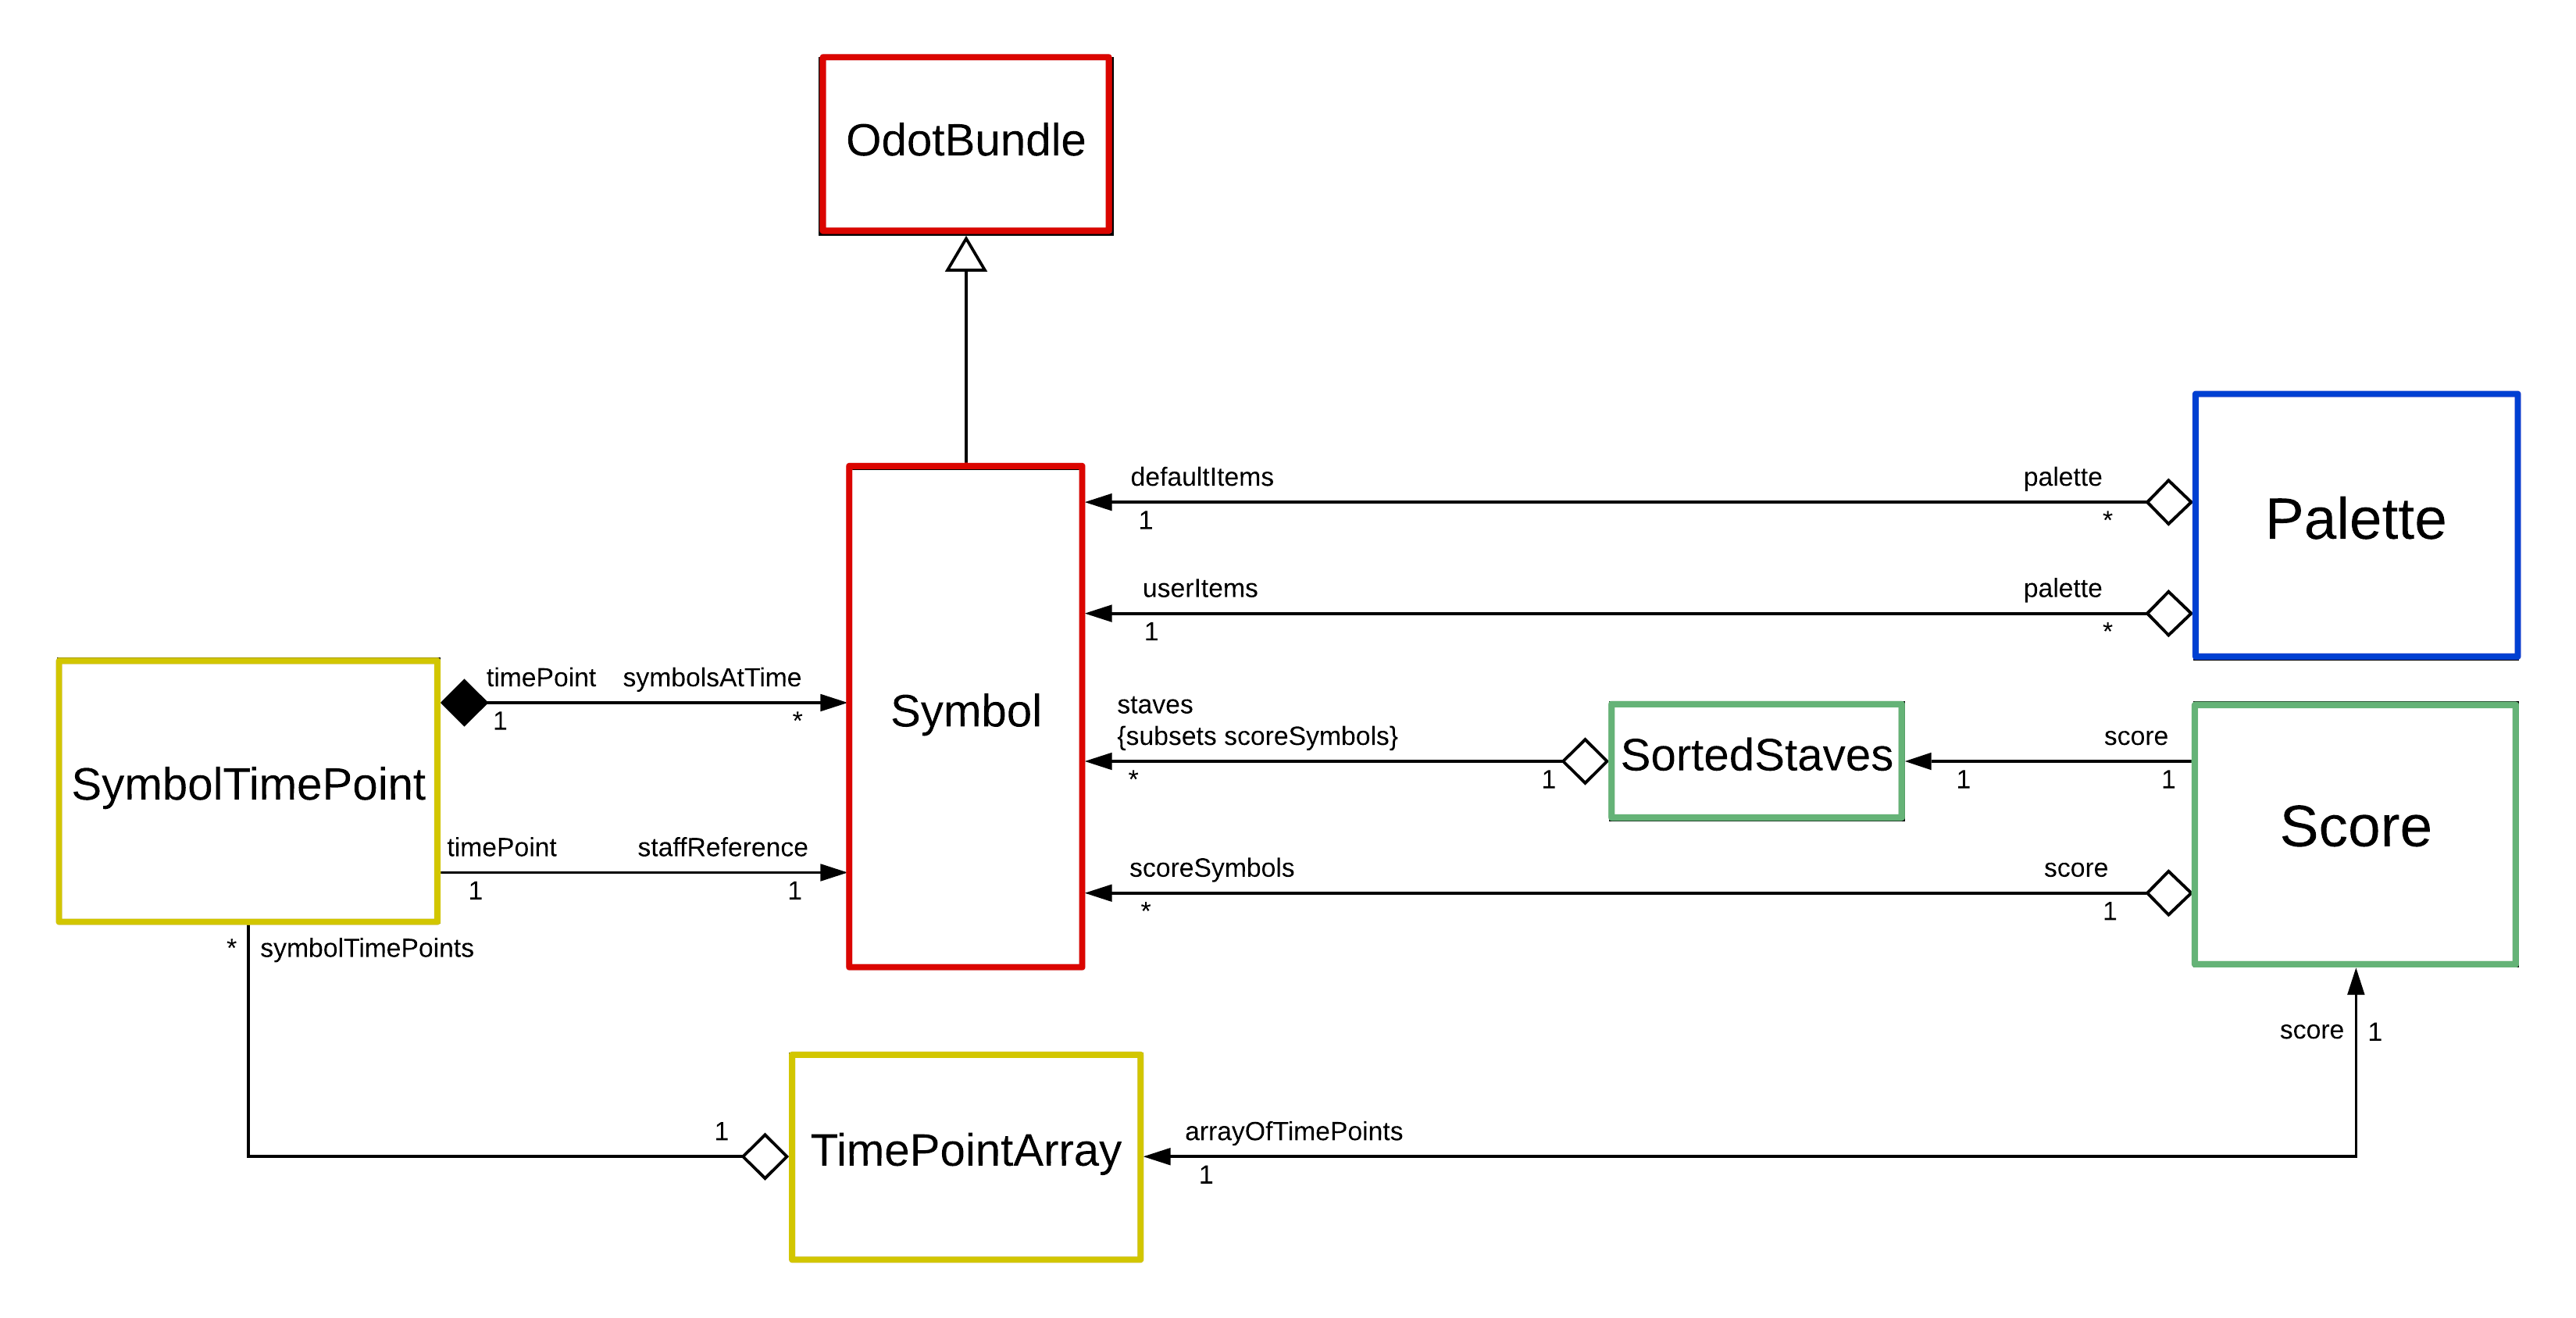
\includegraphics[keepaspectratio=true, width=\textwidth]{Annexes/i/symbolistModelClassDiagram.png}
		\captionof{figure}{Diagramme de classes pour le modèle de l'application symbolist}
		\label{fig:symbolistModelClassDiagram}	
		\medskip
		\small
		\it
		En \textcolor{red}{rouge}, la classe \emph{OdotBundle}, qui encapsule la structure d'un bundle \emph{OSC}, et la classe \emph{Symbol} dont les instances représentent les symboles de la partition. Chaque symbole de la partition possède une structure de bundle OSC, d'où la relation d'héritage entre la classe \emph{OdotBundle} et \emph{Symbol}.
		En \textcolor{blue}{bleu}, la classe \emph{Palette}, regroupant les symboles pouvant être dessinés sur la partition, qu'ils aient été définis par l'utilisateur ou existaient par défaut dans l'application.
		En \textcolor{green}{vert}, les classes \emph{Score} et \emph{SortedStaves} décrivant les symboles présent dans la partition.
		En \textcolor{yellow}{jaune}, les classes \emph{SymbolTimePoint} et \emph{TimePointArray} définissant la logique d'ordonnancement temporel des symboles associés à un \emph{staff}.  
	\end{minipage}
}
\clearpage

\rotatebox{90}{
	\begin{minipage}{0.85\textheight}
		\section{Architecture finale de l'application symbolist}
		\label{sec:symbolistFinalStructure}
		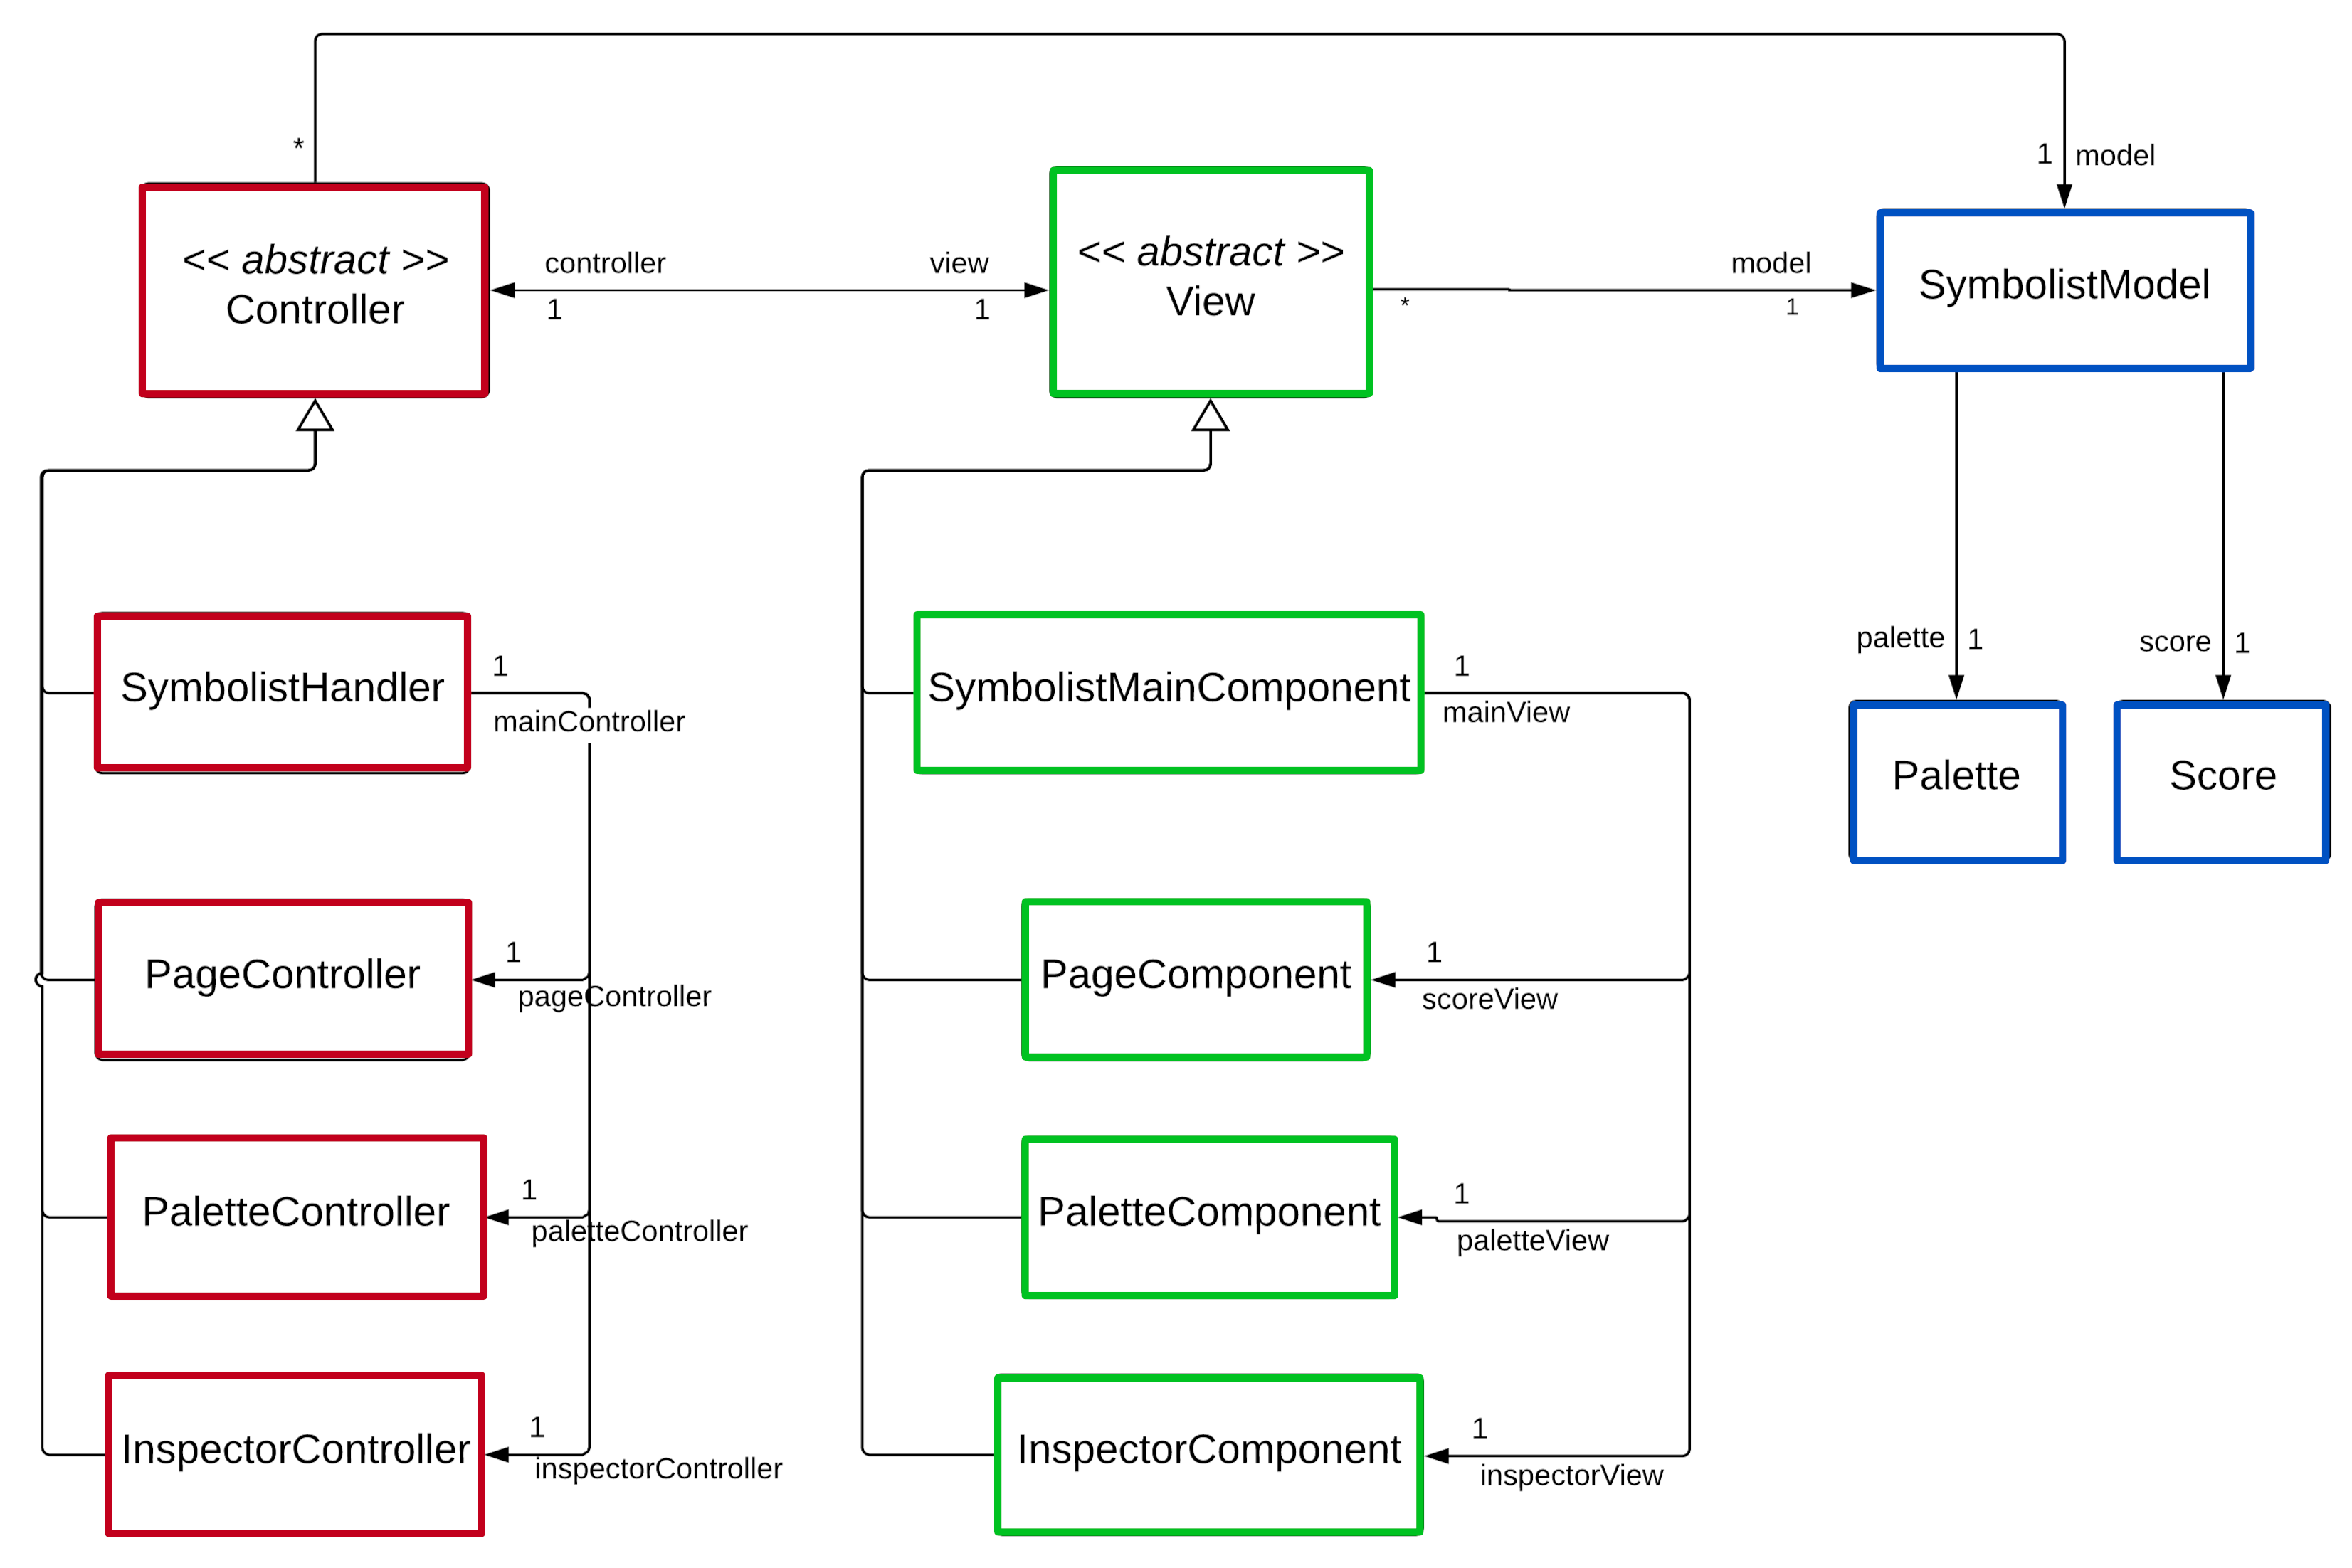
\includegraphics[keepaspectratio=true, width=\textwidth]{Annexes/i/symbolistFinalStructure.png}
		\captionof{figure}{Diagramme de classes présentant l'architecture de l'application symbolist après restructuration}
		\label{fig:symbolistFinalStructure}	
		\medskip
		\small
		\it
		En \textcolor{red}{rouge}, .
		En \textcolor{blue}{bleu}, .
		En \textcolor{green}{vert}, .  
	\end{minipage}
}
\clearpage
